\documentclass[svgnames]{article}
\usepackage[utf8]{inputenc}
\usepackage{amsmath}
\usepackage{amssymb}
\usepackage{mathrsfs}
\usepackage{mathtools}
\newtheorem{mydef}{Given}
\newtheorem{mytheorem}{Theorem}
\usepackage{enumitem}
\usepackage{venndiagram}
\usepackage{smartdiagram}
\usepackage{caption}
\usepackage{subcaption}
%\usepackage[framed,numbered,autolinebreaks,useliterate]{mcode}
\usepackage{pgfplots}
%\usepackage{tkiz}
\usepackage{listings}
\definecolor{dkgreen}{rgb}{0,0.6,0}
\definecolor{gray}{rgb}{0.5,0.5,0.5}
\definecolor{mauve}{rgb}{0.58,0,0.82}
\usepackage{float}
\usepackage{graphicx}
\graphicspath{ {./images/} }

\lstset{ %
  language=R,                     % the language of the code
  basicstyle=\footnotesize,       % the size of the fonts that are used for the code
  numbers=left,                   % where to put the line-numbers
  numberstyle=\tiny\color{gray},  % the style that is used for the line-numbers
  stepnumber=1,                   % the step between two line-numbers. If it's 1, each line
                                  % will be numbered
  numbersep=5pt,                  % how far the line-numbers are from the code
  backgroundcolor=\color{white},  % choose the background color. You must add \usepackage{color}
  showspaces=false,               % show spaces adding particular underscores
  showstringspaces=false,         % underline spaces within strings
  showtabs=false,                 % show tabs within strings adding particular underscores
  frame=single,                   % adds a frame around the code
  rulecolor=\color{black},        % if not set, the frame-color may be changed on line-breaks within not-black text (e.g. commens (green here))
  tabsize=2,                      % sets default tabsize to 2 spaces
  captionpos=b,                   % sets the caption-position to bottom
  breaklines=true,                % sets automatic line breaking
  breakatwhitespace=false,        % sets if automatic breaks should only happen at whitespace
  title=\lstname,                 % show the filename of files included with \lstinputlisting;
                                  % also try caption instead of title
  keywordstyle=\color{blue},      % keyword style
  commentstyle=\color{dkgreen},   % comment style
  stringstyle=\color{mauve},      % string literal style
  escapeinside={\%*}{*)},         % if you want to add a comment within your code
  morekeywords={*,...}            % if you want to add more keywords to the set
} 


%\renewcommand{\theenumi}{\Alph{enumi}}
\newenvironment{amatrix}[1]{%
  \left(\begin{array}{@{}*{#1}{c}|c@{}}
}{%
  \end{array}\right)
}

\newenvironment{tolerant}[1]{%
  \par\tolerance=#1\relax
}{%
  \par
}


\pgfmathdeclarefunction{gauss}{2}{%
  \pgfmathparse{1/(#2*sqrt(2*pi))*exp(-((x-#1)^2)/(2*#2^2))}%
}


\title{Statistical methods: Homework 12}
\author{Cameron McIntyre}
\date{\today}

\begin{document}

\maketitle

\section{11.2.18}

We are given that the distribution of $\theta$ is described by the PMF.

$$P(\theta | n ,k) = \frac{\Gamma (n + r +s)}{\Gamma(r+k)\Gamma(s+ n - k)}\theta^{r + k -1}(1-\theta)^{n+s-k-1}$$

\begin{enumerate}[label = \alph*.]

\item Plot prior and posterior distributions for all 4 cases defined by the following values for parameters: $(r,s)=(1,1),(4,4)\&(n,k)= (4,3),(20,11)$.
\newline
The distribution being used in this case is the conjugate prior of the gamma distribution.

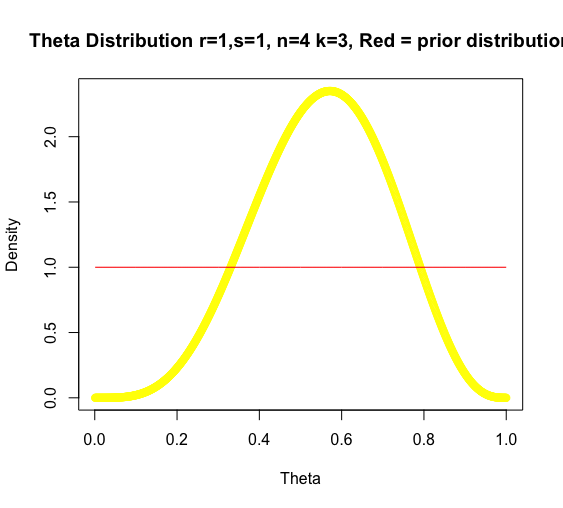
\includegraphics[scale=.5]{1-1-4-3}
$$$$
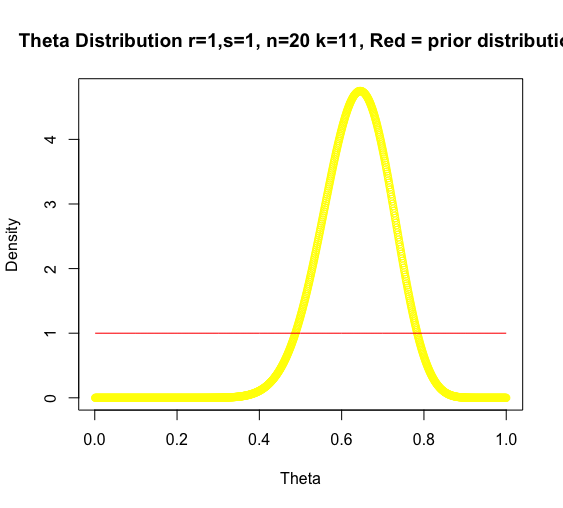
\includegraphics[scale=.5]{1-1-20-11}
$$$$
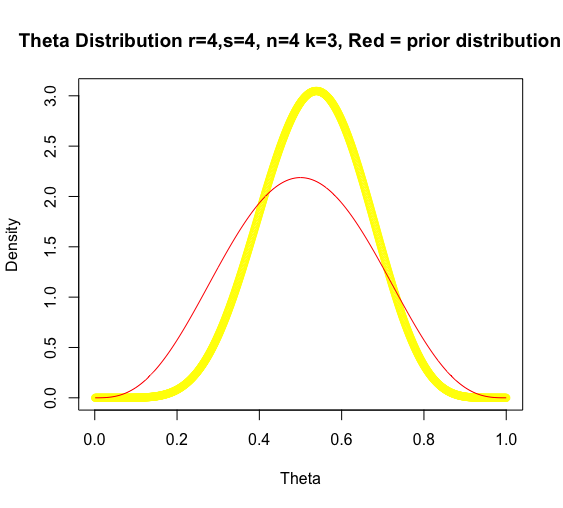
\includegraphics[scale=.5]{4-4-4-3}
$$$$
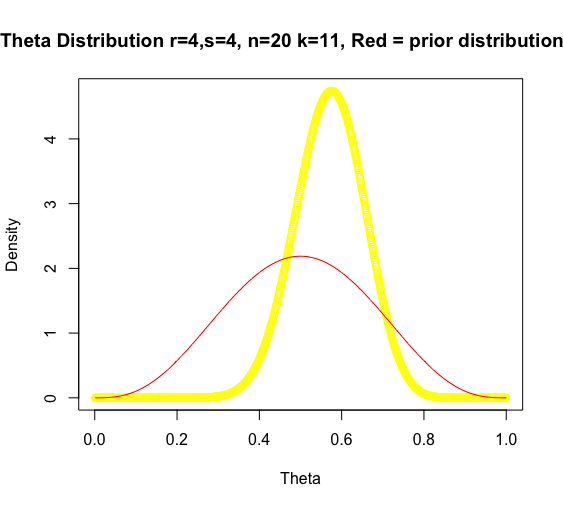
\includegraphics[scale=.5]{4-4-20-11}
\begin{lstlisting}
##r s (1,1) (4,4)
##n k  (4,3) (20,11)


plot(c(1:1000)/1000,dbeta(c(1:1000)/1000,5, 4), col = 103, add = TRUE, xlab = 'Theta', ylab = 'Density', title('Theta Distribution r=1,s=1, n=4 k=3, Red = prior distribution') )
lines(c(1:1000)/1000,dbeta(c(1:1000)/1000,1, 1), col = 26,bg=405)

plot(c(1:1000)/1000,dbeta(c(1:1000)/1000,21, 12), col = 103, add = TRUE, xlab = 'Theta', ylab = 'Density', title('Theta Distribution r=1,s=1, n=20 k=11, Red = prior distribution') )
lines(c(1:1000)/1000,dbeta(c(1:1000)/1000,1, 1), col = 26,bg=405)

plot(c(1:1000)/1000,dbeta(c(1:1000)/1000,8, 7), col = 103, add = TRUE, xlab = 'Theta', ylab = 'Density', title('Theta Distribution r=4,s=4, n=4 k=3, Red = prior distribution    ') )
lines(c(1:1000)/1000,dbeta(c(1:1000)/1000,4, 4), col = 26,bg=405)


plot(c(1:1000)/1000,dbeta(c(1:1000)/1000,24, 15), col = 103, add = TRUE, xlab = 'Theta', ylab = 'Density', title('Theta Distribution r=4,s=4, n=20 k=11, Red = prior distribution       ') )
lines(c(1:1000)/1000,dbeta(c(1:1000)/1000,4, 4), col = 26,bg=405)
\end{lstlisting}

\item  In each one of these 4 cases, determine the probability that the coin is biased towards heads (ie $P(\theta>0.5)$) (You can use Beta distribution integration functionality of R)


\begin{lstlisting}
$$P(\theta>.5 | r=1 ,s=1 ,n= 4, k=3)=0.6367187$$
> 1-pbeta(.5,5, 4)
[1] 0.6367187
\end{lstlisting} 
$$P(\theta>.5 | r=1 ,s=1 ,n= 20, k=11)=0.9449079$$
\begin{lstlisting}
> 1-pbeta(.5,21, 12)
[1] 0.9449079
\end{lstlisting}
$$P(\theta>.5 | r=4 ,s=4, n= 4, k=3)=0.6047363$$
\begin{lstlisting}
> 1-pbeta(.5,8, 7)
[1] 0.6047363
\end{lstlisting} 
$$P(\theta>.5 | r=4 ,s=4, n= 20, k=11)=0.9283467$$
\begin{lstlisting}
> 1-pbeta(.5,24,15)
[1] 0.9283467
\end{lstlisting}
\end{enumerate}
\end{document}
